\documentclass[11pt]{standalone}
\usepackage{amssymb}
\usepackage{amsmath}
\usepackage[no-math]{fontspec}
\usepackage{unicode-math}
\usepackage{libertinus}
\usepackage{pgf,xcolor}
\usepackage{tikz}
\usetikzlibrary{arrows.meta, backgrounds}
\usepackage{pgfplots}
\pgfplotsset{compat=newest}

\definecolor{my_darkgray}{HTML}{484949}
\definecolor{my_lightgray}{HTML}{F3F4F4}
\definecolor{my_darkblue}{HTML}{005A94}
\definecolor{my_lightblue}{HTML}{CCDEE9}
\definecolor{my_yellow}{HTML}{FFEC7F}
\definecolor{my_red}{HTML}{E60000}
\definecolor{my_orange}{HTML}{E87846}

\begin{document}
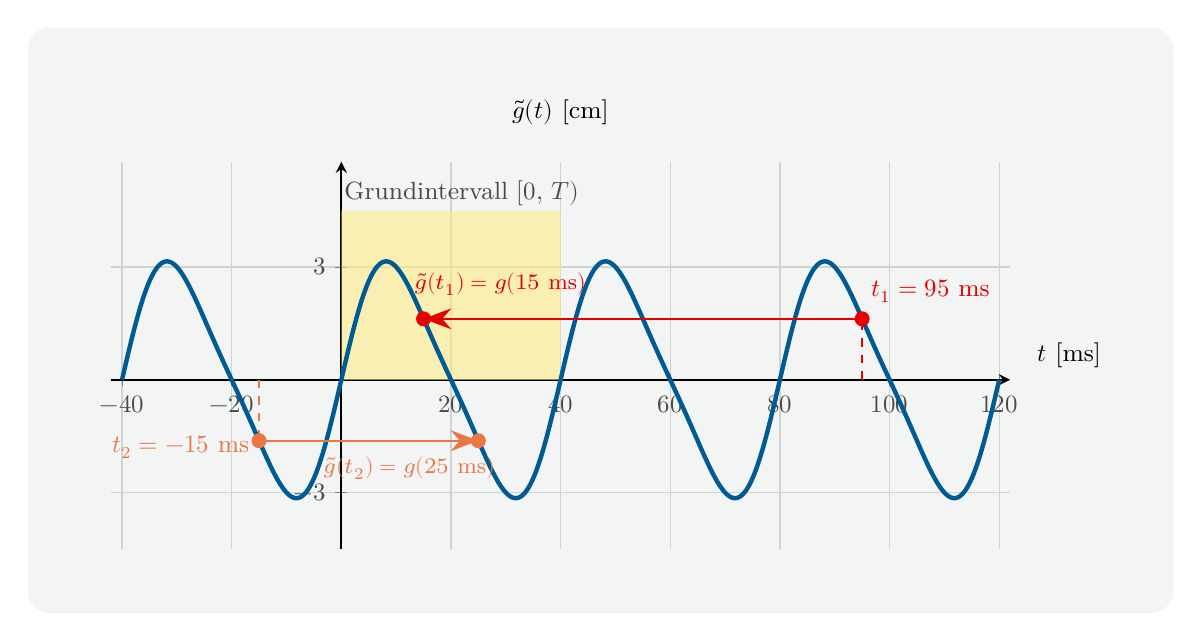
\begin{tikzpicture}[
    show background rectangle,
    background rectangle/.style={fill=my_lightgray, rounded corners=8pt},
    inner frame sep=0.8cm
]

\begin{axis}[
    axis lines = center,
    xlabel = {$t$ [ms]},
    ylabel = {$\tilde{g}(t)$ [cm]},
    xlabel style={at={(axis description cs:1.02,0.5)}, anchor=west, font=\small},
    ylabel style={at={(axis description cs:0.5,1.07)}, anchor=south, font=\small},
    xmin = -42,
    xmax = 122,
    ymin = -4.5,
    ymax = 5.8,
    xtick = {-40, -20, 0, 20, 40, 60, 80, 100, 120},
    xticklabels = {$-40$, $-20$, $0$, $20$, $40$, $60$, $80$, $100$, $120$},
    ytick = {-3, 0, 3},
    yticklabels = {$-3$, $0$, $3$},
    axis line style = {thick},
    grid = both,
    grid style = {draw=my_lightgray!60!white, line width=0.4pt},
    major grid style = {draw=my_lightgray!80!my_darkgray, line width=0.5pt},
    tick label style = {font=\small, color=my_darkgray},
    width = 13cm,
    height = 6.5cm,
    % axis equal not used: time axis (ms) vs displacement (cm) have different units
    clip = false,
]

%% Yellow fill: base interval [0, 40) highlighted behind the curve.
%% We use \fill in the axis coordinate system via addplot fill.
\addplot[
    fill = my_yellow,
    fill opacity = 0.55,
    draw = none,
    domain = 0:40,
    samples = 2,
]{ 4.5 } \closedcycle;

%% Label for the base interval
\node[anchor=north, font=\small, color=my_darkgray]
    at (axis cs: 22, 5.55) {Grundintervall $[0,\,T)$};

%% g(t) = 3*sin(2*pi/T * t) + 0.5*sin(4*pi/T * t)  with T=40 ms, t in ms
%% = 3*sin(pi*t/20) + 0.5*sin(pi*t/10)
%% Periodic continuation: use modular arithmetic via the pgfplots domain trick.
%% We plot each period separately so the curve segments tile correctly.

%% Period k = -1: t in [-40, 0)  -> g(t + 40)
\addplot[
    draw = my_darkblue,
    samples = 150,
    ultra thick,
    domain = -40:0,
]{ 3*sin(deg(pi*(x+40)/20)) + 0.5*sin(deg(pi*(x+40)/10)) };

%% Period k = 0: t in [0, 40)  -> g(t)  (base interval)
\addplot[
    draw = my_darkblue,
    samples = 150,
    ultra thick,
    domain = 0:40,
]{ 3*sin(deg(pi*x/20)) + 0.5*sin(deg(pi*x/10)) };

%% Period k = 1: t in [40, 80)  -> g(t - 40)
\addplot[
    draw = my_darkblue,
    samples = 150,
    ultra thick,
    domain = 40:80,
]{ 3*sin(deg(pi*(x-40)/20)) + 0.5*sin(deg(pi*(x-40)/10)) };

%% Period k = 2: t in [80, 120)  -> g(t - 80)
\addplot[
    draw = my_darkblue,
    samples = 150,
    ultra thick,
    domain = 80:120,
]{ 3*sin(deg(pi*(x-80)/20)) + 0.5*sin(deg(pi*(x-80)/10)) };

%% --- Evaluation point t1 = 95 ms ---
%% Reduced time: 95 - 2*40 = 15 ms  ->  g(15)
%% g(15) = 3*sin(pi*15/20) + 0.5*sin(pi*15/10)
%%       = 3*sin(3*pi/4) + 0.5*sin(3*pi/2)
%%       = 3*(sqrt(2)/2) + 0.5*(-1) ≈ 2.121 - 0.5 = 1.621

% Vertical marker at t1 = 95
\draw[thick, color=my_red, dashed]
    (axis cs: 95, 0) -- (axis cs: 95, 1.621);

% Dot at the function value
\addplot[
    only marks,
    mark = *,
    mark size = 2.5pt,
    color = my_red,
]
coordinates { (95, 1.621) };

% Arrow pointing from t1=95 back to reduced time t=15
\draw[-{Stealth[length=10pt]}, thick, color=my_red]
    (axis cs: 95, 1.621) -- (axis cs: 15, 1.621);

% Dot at reduced time t=15 on base interval
\addplot[
    only marks,
    mark = *,
    mark size = 2.5pt,
    color = my_red,
]
coordinates { (15, 1.621) };

% Labels for t1
\node[anchor=south west, font=\small, color=my_red]
    at (axis cs: 95, 1.8) {$t_1 = 95~\text{ms}$};

\node[anchor=north, font=\footnotesize, color=my_red]
    at (axis cs: 29, 3.1) {$\tilde{g}(t_1) = g(15~\text{ms})$};

%% --- Evaluation point t2 = -15 ms ---
%% Reduced time: -15 + 40 = 25 ms  ->  g(25)
%% g(25) = 3*sin(pi*25/20) + 0.5*sin(pi*25/10)
%%       = 3*sin(5*pi/4) + 0.5*sin(5*pi/2)
%%       = 3*(-sqrt(2)/2) + 0.5*(1) ≈ -2.121 + 0.5 = -1.621

% Vertical marker at t2 = -15
\draw[thick, color=my_orange, dashed]
    (axis cs: -15, 0) -- (axis cs: -15, -1.621);

% Dot at the function value
\addplot[
    only marks,
    mark = *,
    mark size = 2.5pt,
    color = my_orange,
]
coordinates { (-15, -1.621) };

% Arrow pointing from t2=-15 forward to reduced time t=25
\draw[-{Stealth[length=10pt]}, thick, color=my_orange]
    (axis cs: -15, -1.621) -- (axis cs: 25, -1.621);

% Dot at reduced time t=25 on base interval
\addplot[
    only marks,
    mark = *,
    mark size = 2.5pt,
    color = my_orange,
]
coordinates { (25, -1.621) };

% Labels for t2
\node[anchor=east, font=\small, color=my_orange]
    at (axis cs: -15, -1.8) {$t_2 = -15~\text{ms}$};

\node[anchor=north west, font=\footnotesize, color=my_orange]
    at (axis cs: -5, -1.8) {$\tilde{g}(t_2) = g(25~\text{ms})$};

\end{axis}

\end{tikzpicture}
\end{document}
